\section{Методология}
\subsection{Введение}
Как было описано выше, проект был разделен на две части, которые реализовывались отдельно друг от друга, однако они обе имеют общую часть предобработки изображений.

Важно ещё раз отметить, что подход с использованием EM алгоритма разрабатывался в сжатые сроки, являясь временным решением, что, однако, не снимало с него требований 
на точность в детекции канала, хотя это требование не было критическим, т.е. алгоритм мог выдавать шумные маски. 
\subsection{Подход без глубокого обучения}
Для сегментации без использования глубокого обучения использовался EM алгоритм. В него подавалось предобработанное изображение целиком, после чего алгоритм приписывал
каждому пикселю метку класса, основываясь только на цвете пикселя. После чего происходила фильтрация маски (этот процесс описан в конце главы). Данный подход выдавал 
шумные маски, однако даже они позволили начать собирать информацию о ледяном канале в дневное время суток.
\subsubsection{EM алгоритм}
\noindent \textbf{Простой случай}
\\
Предположим есть несколько точек в $d$-мерном пространстве, это наши данные, задача их сегментировать.
\begin{figure}[ht]
    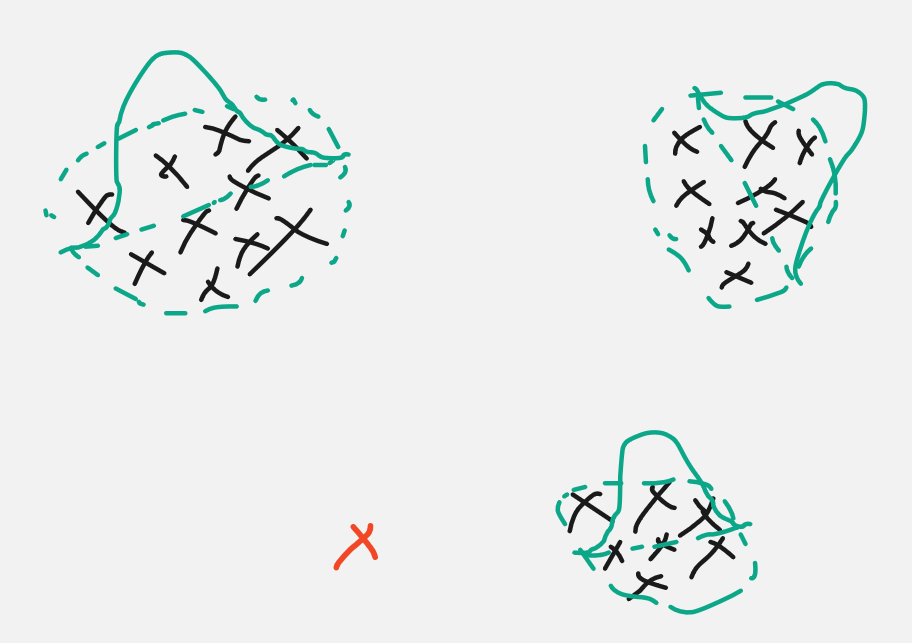
\includegraphics[scale=0.5]{src/Design/assets/em_picture.png}
    \caption{Данные в простом случае}
\end{figure}
Положим, что данные были порождены смесью трёх гауссианов:
\[p(\overline{x}) = \pi_1\cdot p_1(\overline{x}) + \pi_2\cdot p_2(\overline{x}) + \pi_3\cdot p_3(\overline{x}) \]
где
\[\sum\limits_{k=1}^{K} \pi_k = 1 \text{, где } K=3\]
Другими словами, с вероятностью $\pi_i$ будет выбран i-ый гауссиан, после чего будут сгенерированы точки данных на основе этого распределения. 
$\overline{x} \sim p_k(\overline{x})$.
Но возникает вопрос, к какому кластеру отнести новую точку (красную)?
Для этого необходима функция правдоподобия: \\
$\displaystyle p(D|\overline{\theta}) = \prod\limits_{n=1}^N p(\overline{x}_n | \overline{\theta})$ здесь $D$ обозначает весь датасет, другими словами \\$D = \{\overline{x}_n \} _{n=1}^N$
\\
Где
\[p(\overline{x} | \overline{\theta}) = \sum\pi_k\cdotp_k(\overline{x}) = \sum\limits_{k}\pi_k\cdot\mathcal{N}(\overline{x}|\overline{\mu}_k, \Sigma_k)\]
Где $\overline{\mu}_i \text{ и } \Sigma_i$ --- параметры плотности нормального распределения, а

\[\overline{\theta} = (\pi_1, \dots \pi_K,
\overline{\mu}_1, \Sigma_1, \dots, \overline{\mu}_K, \Sigma_K)\] 
После чего:
\[p(D|\overline{\theta}) = \prod\limits_{n=1}^N p(\overline{x}_n | \overline{\theta}) =
 \prod\limits_{n=1}^N (\pi_1\cdot p_1(\overline{x}_n | \overline{\theta}_1) + \pi_2\cdot p_2(\overline{x}_n | \overline{\theta}_2) + 
 \dots + \pi_K\cdot p_K(\overline{x}_n | \overline{\theta}_K) ) \overset{}{\underset{\overline{\theta}}{\rightarrow}} \text{max}\]
 Где $\overline{\theta}_i = (\overline{\mu}_i, \Sigma_i)$
\\
Проблема в том, что это произведение большого числа сумм, из-за чего это сложно максимизировать
Идея в том, чтобы посмотреть на распределение, правдоподобие и порождающий процесс и понять, какая еще информация об этом процессе необходима, чтобы
облегчить максимизацию правдоподобия.
\\
Оказывается, что добавление к $\overline{x}$ меток класса сильно облегчает максимизацию. В математическом виде это можно представить так:

\[ Z = \{\overline{z}_n \} _{n=1}^N \text{, где каждый } \overline{z}_n \text{ в one-hot представлении: } \overline{z}_n = (0,\dots,1,\dots0)\] 
% and only 1 of this vector is on the kth position, which means that $x_n \in C_k$, where $C_k$ means cluster number k.
% So if $Z$ is known, then
Поэтому если $Z$ известно, то
\[p(D, Z | \overline{\theta}) = \prod\limits_{n=1}^{N}p(\overline{x}_n, \overline{z}_n | \overline{\theta})
= \prod\limits_{n=1}^{N}p(\overline{z}_n | \overline{\pi})\cdot p(\overline{x}_n| \overline{z}_n, \overline{\theta})
= \prod\limits_{n=1}^{N}\prod\limits_{k=1}^{K}{(\pi_k\cdot\mathcal{N}(\overline{x}_n|\overline{\mu}_k,\Sigma_k))}^{{z_n}_k}\]

\[\log(p(D, Z | \overline{\theta})) = \sum\limits_{n=1}^{N}\sum\limits_{k=1}^{K}{z_n}_k \cdot (\log(\pi_k) +  \log(\mathcal{N}(\overline{x}_n|\overline{\mu}_k,\Sigma_k)))\]
\[= \sum\limits_{k=1}^K \log(\pi_k) \cdot \sum\limits_{n=1}^N {z_n}_k + 
\sum\limits_{k=1}^K \big( \sum\limits_{n=1}^N {z_n}_k \cdot \log(\mathcal{N}(\overline{x}_n|\overline{\mu}_k,\Sigma_k)) \big)\]
Можно заметить, что первое и второе слагаемые зависят от разных параметров.
Первое слагаемое зависит от $\pi_k$, а второе от параметров плотности нормального распределения $\overline{\mu}_k, \Sigma_k$. Это даёт возможность максимизировать слагаемые независимо.
\\
И главная идея в следующем. Сложная функция правдоподобия становится простой, если известны скрытые параметры ($Z$). 
Поэтому процесс максимизации можно разбить на два шага 
\begin{enumerate}
    \item E-шаг (зафиксировать $\overline{\theta}$, найти $\mathbb{E}[Z]$):
    \[\mathbb{E}[z_{n, k}] = p(C_k|\overline{x}_n,\overline{\theta}) 
    = \displaystyle \frac{p(C_k|\overline{\theta})\cdot p(\overline{x}_n|C_k,\overline{\theta})}{\sum\limits_{l=1}^K p(C_l|\overline{\theta})\cdot p(\overline{x}_n|C_l,\overline{\theta})}
    = \displaystyle \frac{\pi_k\cdot \mathcal{N}(\bar x_n | \bar \mu_k, \Sigma_k)}{\sum\limits_{l=1}^K \pi_l \cdot \mathcal{N}(\bar x_n | \bar \mu_l, \Sigma_l)}\]
    \item M-шаг (зафиксировать $\mathbb{E}[Z]$, максимизировать $\mathbb{E}[\log(p(D,Z|\overline{\theta}))]$). В большинстве случаев вместо $Z$, можно использовать его мягкие оценки $\mathbb{E}(Z)$:
    \[\mathbb{E}[\log p(D,Z|\bar\theta)] 
    = \mathbb{E}\Big[\sum\limits_n\sum\limits_k {z_n}_k \cdot \big(\log(p(\overline{x}_n|\overline{\mu}_k, \Sigma_k)) + \log(\pi_k)\big)\Big]\] 
    \[ = \sum\limits_n\sum\limits_k\mathbb{E}[{z_n}_k]\cdot(\log(\pi_k) + \log\big(p(\overline{x}_n|\overline{\mu}_k, \Sigma_k)))\]
    \[= \sum\limits_k\Big(\sum\limits_n\mathbb{E}[z_{n,k}]\Big) \log \pi_k + \sum\limits_k\sum\limits_n\mathbb{E}[z_{n,k}]\cdot \log p(\bar x_n|\bar\mu_k,\Sigma_k)\]
\end{enumerate}

\noindent\textbf{Общий случай}
\\
Даны:
\begin{enumerate}
    \item X \- датасет
    \item Z \- скрытые параметры (они неизвестны)
    \item $\theta$ \- параметры модели, которые тоже неизвестны
\end{enumerate}
Задача --- максимизировать $p(X|\theta)$, что является сложной задачей, однако максимизация $p(X, Z|\theta)$ сильно легче. Поэтому пусть
\[Q(\theta, \theta^{(n)}) := \mathbb{E}_{p(Z|X,\theta^{(n)})} \big[\log p(X,Z|\theta)\big]
= \int \log p(X,Z|\theta) \cdot p(Z|X,\theta^{(n)}) dz \]
И на каждой итерации:
\[\theta^{(n+1)} = \underset{\theta}{\mathrm{argmax }}\text{ } Q(\theta, \theta^{(n)})\]
\\
Итерации продолжаются до тех пор пока $\theta$ или правдоподобие не перестанут меняться (теоретически это должно произойти одновременно). 
Также стоит отметить, что правдоподобие должно только увеличиваться после каждой итерации. Поэтому имеем:
\[\log(p(X|\theta)) > \log(p(X|\theta^{(n)}))\]
\[\log(p(X|\theta)) - \log(p(X|\theta^{(n)})) 
= \log \Big( \int p(X,Z|\theta) dz \Big) - \log(p(X|\theta^{(n)})) \]
\[= \log \Big(\int p(Z|X,\theta^{(n)} \cdot \displaystyle \frac{p(X,Z|\theta)}{p(Z|X,\theta^{(n)})}) dz \Big) - \log(p(X|\theta^{(n)}))\]
\[= \log\Big( \mathbb{E}_{p(Z|X,\theta^{(n)})}\big[\displaystyle\frac{p(X,Z|\theta)}{p(Z|X,\theta^{(n)})} \big] \Big) - \log(p(X|\theta^{(n)})) \]
\[ \underset{\text{по неравенству Йенсена}}{\geq} \mathbb{E}_{p(Z|X,\theta^{(n)})}\Big[\log\big(\displaystyle\frac{p(X,Z|\theta)}{p(Z|X,\theta^{(n)})} \big) \Big]  - \log(p(X|\theta^{(n)})) \]
\[ = \mathbb{E}_{p(Z|X,\theta^{(n)})}\Big[\log\big(\displaystyle\frac{p(X,Z|\theta)}{p(Z|X,\theta^{(n)}) \cdot p(X|\theta^{(n)})} \big) \Big]\]
Важно заметить, что $p(Z|X,\theta^{(n)}) \cdot p(X|\theta^{(n)}) = p(X,Z|\theta^{(n)})$

\noindent И поэтому:
\[ \log(p(X|\theta)) \geq \log(p(X|\theta^{(n)})) + \mathbb{E}_{p(Z|X,\theta^{(n)})}\Big[\log\big(\displaystyle\frac{p(X,Z|\theta)}{p(Z|X,\theta^{(n)}) \cdot p(X|\theta^{(n)})} \big) \Big] =: \mathcal{L}(\theta, \theta^{(n)})\]

\begin{figure}[h]
    \begin{center}
        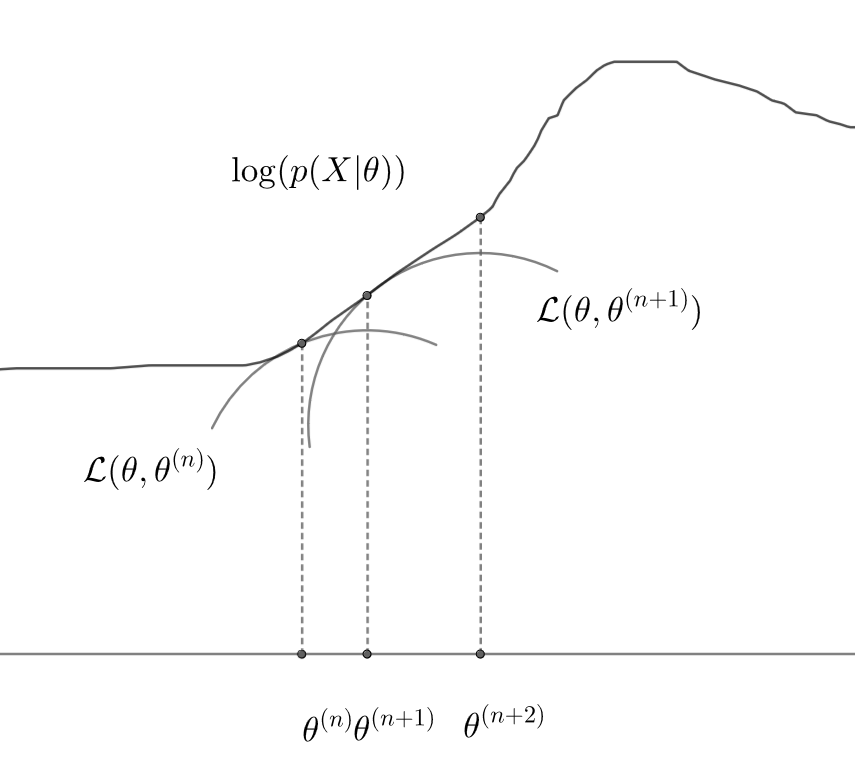
\includegraphics[scale=0.45]{src/Design/assets/em_visualisation.png}
    \end{center}
    \caption{Визуализация алгоритма}\label{fig:em_visual}
\end{figure}

\noindent Как показано на Рис.~\ref{fig:em_visual}, в каждой точке  ($\theta^{(n)}$, $\theta^{(n+1)}$, $\theta^{(n+2)}$ и т.д.) известно наименьшее значение $\log(p(X|\theta))$, при этом оно же равно $\mathcal{L}(\theta, \theta^{(n)})$
\\
Также важно заметить, что $\log(p(X|\theta^{(n)})) = \mathcal{L}(\theta^{(n)}, \theta^{(n)})$
\\
Поэтому идея --- оптимизировать $\mathcal{L}(\theta, \theta^{(n)})$. Эта функция сходится к локальному максимуму, что тоже неплохо.
\\
Однако в начале было указано, что необходимо оптимизировать $Q(\theta, \theta^{(n)})$, но оказывается, что оптимизация $Q$ и $\mathcal{L}$ --- это одна и та же задача.
\\
\[ \mathcal{L}(\theta, \theta^{(n)}) = \underset{const(\theta)}{\log(p(X|\theta^{(n)}))} + \underset{\text{это и есть } Q(\theta, \theta^{(n)})}{\mathbb{E}_{p(Z|X,\theta^{(n)})}\Big[\log\big(p(X,Z|\theta) \big) \Big]}\]
\[- \underset{const(\theta)}{\mathbb{E}_{p(Z|X,\theta^{(n)})}\Big[\log\big(p(X,Z|\theta^{(n)})\big)\Big]}
    \]

\subsection{Подход с глубоким обучением}
Во втором подходе использовалась следующая архитектура (на Рис~\ref{nn_architecure}):
\begin{enumerate}
    \item Бэкбоун --- сверточная четырехслойная сеть
    \item DINO --- трансформер для извлечения дополнительных фич
    \item Классификатор --- свертка $1\times 1$ с тремя выходными каналами
\end{enumerate}
\begin{figure}[h]
    \begin{center}
        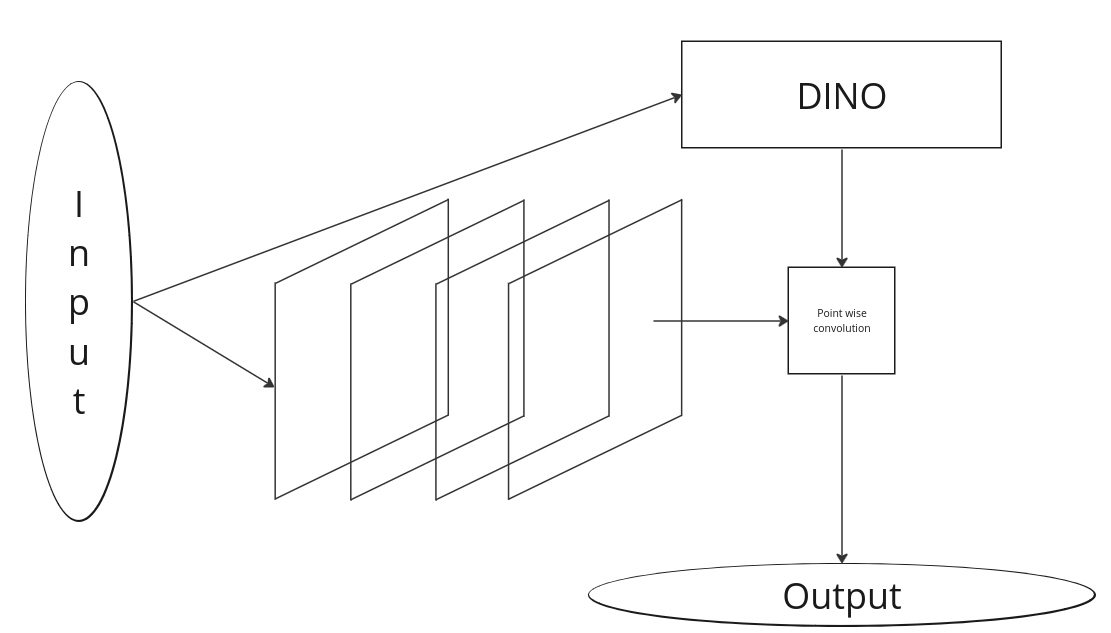
\includegraphics[scale=0.4]{src/Design/assets/NN_architecure.png}
    \end{center}
    \caption{Архитектура нейросети}\label{nn_architecure}
\end{figure}
Было решено создать небольшой датасет и сделать обучение с учителем, предварительно обучив бэкбоун и используя DINO для получения дополнительных признаков 
по всему изображению.
\subsubsection{Бэкбоун}
Бэкбоун обучался на классической задаче решения пазлов, т.е. в бэкбоун подавались части изображения, а на выход ожидался один из четырех классов, 
показывающих расположение части фотографии. Данный подход позволил бэкбоуну научиться извлекать признаки, характерные для изображений датасета, что позволило получить 
относительно неплохие результаты, о которых речь пойдет в следующей главе. В качестве основного блока бэкбоуна использовался стандартный блок из:
\begin{enumerate}
    \item Свертка $3\times 3$
    \item Батч нормализация
    \item ReLU
    \item Дропаут слой
\end{enumerate}

\subsubsection{DINO}
\noindent\textbf{Предпосылки к использованию DINO} \\
DINO --- это архитектура Visual Transformer (ViT) и подход к его обучению. Данная архитектура хорошо себя показывает в извлечении признаков, на основе которых 
можно находить ближайших соседей изображений, что показано в статье про архитектуру STEGO~\cite{stego}. Поэтому было решено включить DINO в итоговую архитектуру, чтобы
улучшить качество сегментации.
\\
\textbf{Архитектура DINO} \\
Основная идея сети --- предсказание выхода учителя, построенного с помощью кодировщика с моментом, используя кросс-энтропию в качестве лосс функции.
\\
В основе DINO лежит архитектура Vision Transformer (ViT), которая обучается без учителя. В DINO используются две сети: ученик и учитель. 
Ученик обновляется на каждом шаге градиента, в то время как веса учителя обновляются с помощью скользящего среднего весов ученика.
\\
Самообучение в DINO происходит следующим образом.
На вход каждой сети подаётся изображение $x$, на выход сети выдают $K$-мерный вектор $P$ с вероятностями (полученный при помощи softmax с температурой):
\[P_s{(x)}^{(i)} = \frac{\exp(g_{\theta_s}{(x)}^{(i)} / \tau_s)}{\sum\limits_{k=1}^K\exp(g_{\theta_s}{(x)}^{(k)} / \tau_s)}\]
\\
Здесь $\tau_s$ --- температура, контролирующая ``остроту'' выхода. Для сети-учителя применяется такое же преобразование.
\\
Далее, учительская сеть замораживается, а сеть-ученик обучается с использованием кросс-энтропии и идеи ``локально-глобального соответствия''. Для этого 
из каждой фотографии входного батча составляется набор искаженных кропов (вырезов или обрезанных частей) изображения $V$. 
При этом в этом наборе содержатся два ``глобальных кропа'' изображения (покрывающих более 50\% изображения): $x_1, x_2$; и несколько локальных кропов. 
Все кропы подаются в сеть-ученик, а в сеть-учитель только глобальные кропы. Затем для обучения сети-ученика минимизируется следующий лосс:
\[\overset{}{\underset{\theta_s}{\min}} \sum\limits_{x\in\{x_1,x_2\}} \sum\limits_{x'\in V; x' \neq x}H(P_t(x), P_s(x'))\]
Где $H(a,b) = -a\cdot\log(b)$
\\
Для обновления весов учительской сети используется следующий подход (важно отметить, что сеть-учитель и сеть-ученик отличаются только весами, 
архитектуры у них одинаковые):
\[\theta_t \leftarrow \lambda \theta_t + (1-\lambda)\cdot \theta_s\]
Где $\lambda$ изменяется по ``косинусному расписанию'' (cosine scheduling) от $0.996$ до $1$.
\\
\noindent Также важно отметить, что многие архитектуры обучения без учителя подвержены вырожденым решениям (когда все кластеризуется в один кластер), чтобы этого не случилось в 
DINO используется центрирование и ``заострение'' при помощи температуры, описанное выше. Эти две техники имеют противоположные эффекты, 
что даёт возможность избежать вырожденного решения. Центрирование смещает сеть ближе к равномерному распределению, в то время как ``заострение'' противодействует этому.
Центрирование можно рассматривать, как смещение (bias) в сети, однако оно обновляется используя экспоненциально скользящее среднее. что кстати нивелирует 
зависимость от размера батча:
\[c\leftarrow mc + (1-m)\frac{1}{B}\sum\limits_{i=1}^B g_{\theta_t}(x_i)\]
\\
Здесь $B$ --- размер батча, а $m$ --- параметр, влияющий на скорость обновления параметра $c$.
\\  
Примерный код обучения DINO представлен в листинге~1~\cite{DINO}


\begin{lstlisting}[label=algo1, language=Python, float=tp, caption={Алгоритм обучения DINO}]
# gs, gt: student and teacher networks
# C: center (K)
# tps, tpt: student and teacher temperatures
# l, m: network and center momentum rates
gt.params = gs.params
for x in loader: # load a minibatch x with n samples
    x1, x2 = augment(x), augment(x) # random views
    s1, s2 = gs(x1), gs(x2) # student output n-by-K
    t1, t2 = gt(x1), gt(x2) # teacher output n-by-K
    loss = H(t1, s2)/2 + H(t2, s1)/2
    loss.backward() # back-propagate
    # student, teacher and center updates
    update(gs) # SGD
    gt.params = l*gt.params + (1-l)*gs.params
    C = m*C + (1-m)*cat([t1, t2]).mean(dim=0)
def H(t, s):
    t = t.detach() # stop gradient
    s = softmax(s / tps, dim=1)
    t = softmax((t - C) / tpt, dim=1) # center + sharpen
    return - (t * log(s)).sum(dim=1).mean()
\end{lstlisting}

\subsubsection{Итоговая сеть}
Как было указано в начале подглавы итоговая сеть в качестве головы имеет свертку $1\times1$. Для обучения этой головы, был размечен небольшой 
датасет на 100 изображений, 80 из которых использовались для обучения, 20 для валидации результата. В качестве лосс функции использовалась стандартная кросс-энтропия:

\[L(x,y) = -w_y \cdot \log\frac{\exp(x_y)}{\sum\limits_{c=1}^C \exp(x_c)}\]
Здесь, $x$ --- выход нейросети, $y$ --- ground-truth метка, а $w$ --- веса для каждого класса. В обучении использовались следующие веса: 10 для воды и ледяного сала, 1 для воды.
В итоговой сети использовался уже предобученный DINO, что позволило увеличить целевые метрики.

\subsubsection{Фильтрация выхода}
Поскольку нейросеть обучалась на небольшом датасете, а многие изображения трудно различимы, то не все ответы нейросети используются. Вместо этого в течение определенного 
небольшого времени алгоритм работает, накапливая результаты, после чего выбирается результат, являющийся медианой всех полученных данных, и именно он считается 
результатом работы алгоритма. В качестве значения, по которому находится медиана, используется ширина канала, которая определяется на основе полученной маски.

Данный подход используется, дабы уменьшить влияние шума и артефактов изображения.

\subsection{Предобработка изображений}

\begin{figure}[htbp]
    \centering
    \subfloat[Изначальное изображение]{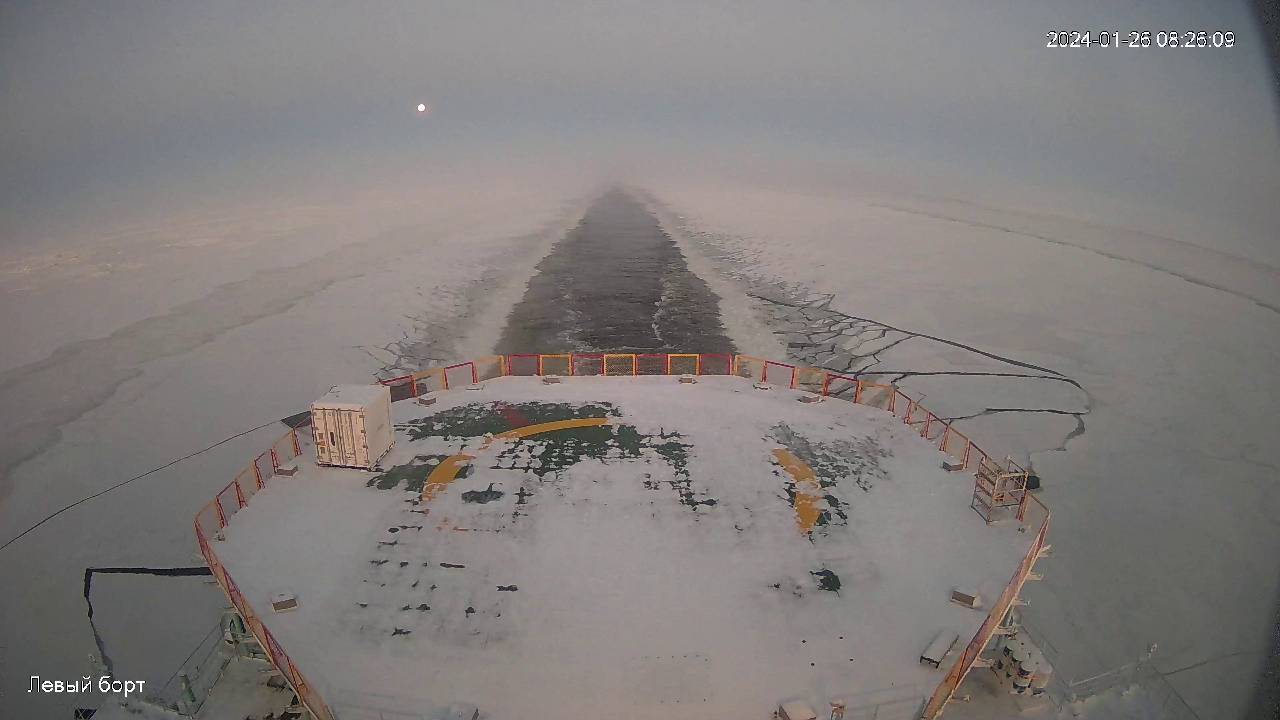
\includegraphics[scale=0.18]{src/Design/assets/raw.png}}
    \subfloat[Компенсация рыбьего глаза]{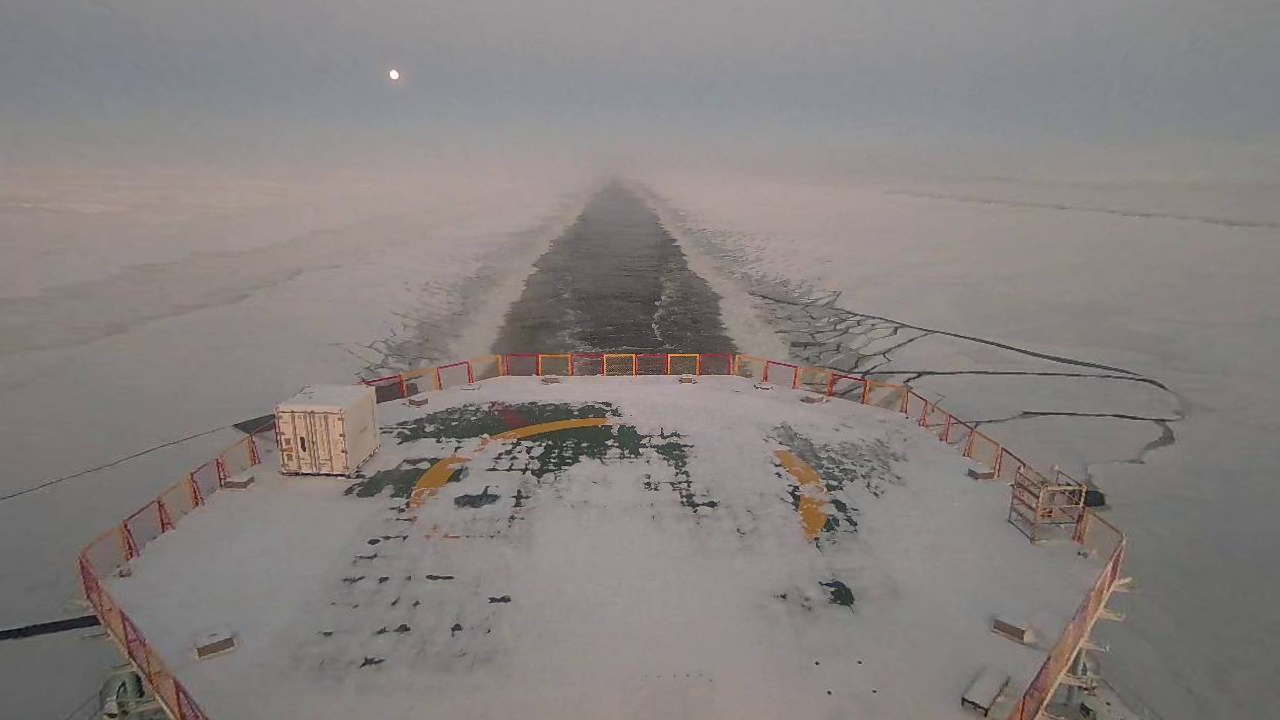
\includegraphics[scale=0.18]{src/Design/assets/undistored.png}}
    \\
    \subfloat[Обрезание по вертикали]{
\includegraphics[scale=0.18]{src/Design/assets/vertical_cropped.png}}
    \subfloat[Повышение контрастности]{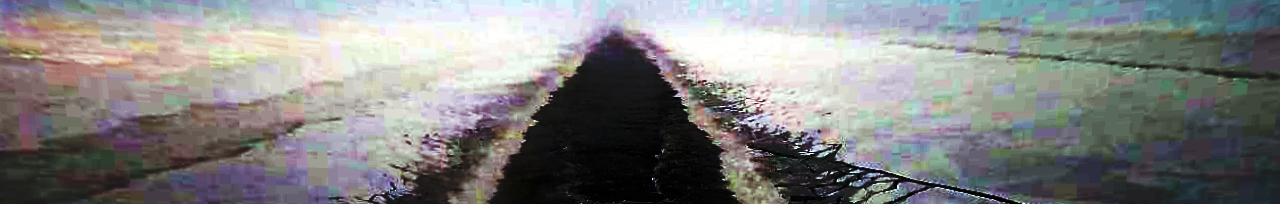
\includegraphics[scale=0.18]{src/Design/assets/equalised.png}}
    \\
    \subfloat[Обрезание по горизонтали]{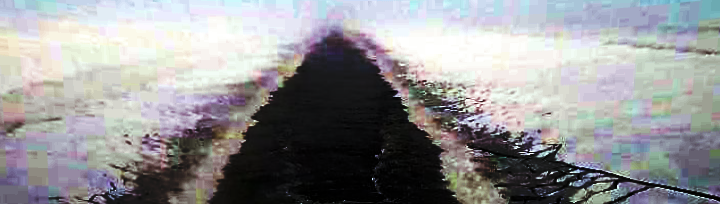
\includegraphics[scale=0.2]{src/Design/assets/horizontal_cropped.png}}
    \caption{Предобработка изображения}\label{fig:preprocessing}
\end{figure}

Этап предобработки изображений одинаков для EM алгоритма и нейросети. Сначала в изображении компенсируется рыбий глаз, вызванный камерой, далее изображение обрезается 
по вертикали. Так как камера установлена статично, то на изображении всегда на одинаковых позиция присутствует как часть кормы судна, так и часть неба. Оба этих 
элемента не имеют отношения к сегментации канала, они, напротив, добавляют сложности к задачи сегментации, поскольку EM алгоритм больше выделяет части судна в 
отдельный кластер, а бэкбоун нейросети больше обучается на признаках судна, нежели на текстуре канала. Исходя из этих наблюдений было решено обрезать эту часть 
изображения. Далее у изображения повышается контрастность, путем выравнивания гистограммы и обрезаются края по горизонтали, так как при повышении контрастности 
они становятся темнее, чем центральная часть изображения, что приводит к неверной сегментации. Такое изображение подается в ЕМ и нейросеть. 

\begin{figure}[htbp]
    \centering
    \subfloat[Маска EM алгоритма]{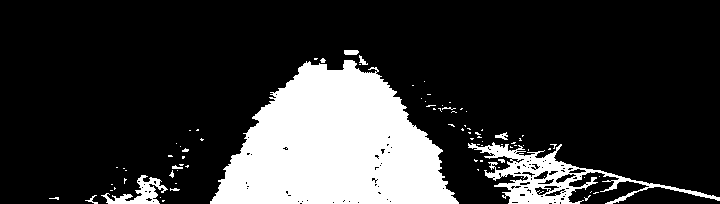
\includegraphics[scale=0.2]{src/Design/assets/em_mask.png}}
    \subfloat[Применение эрозивной фильтрации]{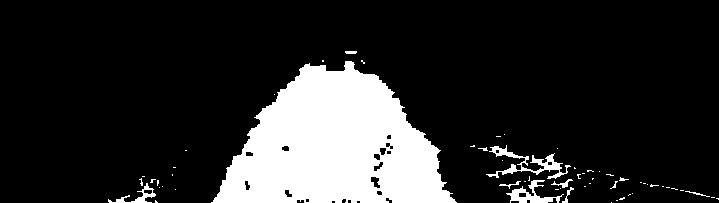
\includegraphics[scale=0.2]{src/Design/assets/morf_mask.png}}
    \\
    \subfloat[Применение BFS для окончательной фильтрации]{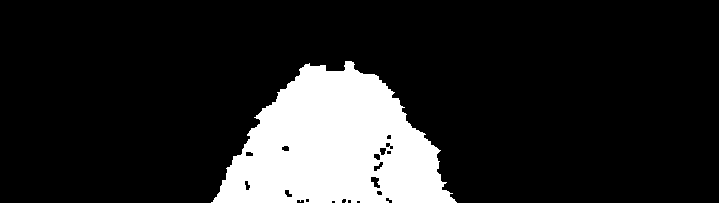
\includegraphics[scale=0.2]{src/Design/assets/bfs_mask.png}}
    \caption{Постобработка маски ЕМ алгоритма}\label{fig:postprocessing}
\end{figure}

В случае ЕМ алгоритма был реализован небольшой постпроцессинг, так как маска, выдаваемая EM алгоритмом, довольно шумная. В первую очередь происходит эрозивная 
фильтрация, чтобы немного избавиться от шума и отделить маску канала от неправильно классифицированных пикселей, после чего применяется поиск в графе. Начальными 
``вершинами'' считаются пиксели, лежащие по центру кадра (там всегда начинается канал), затем в маску добавляются все пиксели отмеченные, как принадлежащие каналу, 
которые являются соседними с уже добавленными в маску. Такой подход позволяет отделить канал от неправильных меток по бокам изображения, которые возникают из-за
изменения яркости картинки после повышения контрастности, что было описано выше.

На Рис.~\ref{fig:preprocessing} приведены этапы предобработки изображений для обоих подходов, а на Рис.~\ref{fig:postprocessing} постобработки 
масок EM алгоритма